\section{Introduction}
\label{section:introduction}

Realistic simulation of driving scenarios is a foundational requirement for the development, training, and evaluation of autonomous driving systems. Generative world models enable scalable and diverse synthetic data creation, reducing reliance on expensive real-world data collection and facilitating robust evaluation in safe and repeatable environments. Unlike general-purpose text-to-video or image-to-video models, which primarily focus on visual realism and temporal coherence, autonomous driving applications demand fine-grained control over domain-specific aspects of the scene.

Generative models for autonomous driving must accurately simulate factors such as the actions of the ego-vehicle, the locations and movements of other agents (e.g., vehicles, pedestrians, cyclists), and their interactions. Moreover, these models must allow conditional generation based on contextual attributes, such as geographic location, weather, time of day, road configuration (e.g., speed limits, number of lanes, pedestrian crossings, traffic lights, intersections), and rare but critical edge-case scenarios. The ability to generate consistent multi-camera video streams is also essential, as autonomous vehicles rely on spatially and temporally coherent input from multiple perspectives for perception and decision-making. Meeting these domain-specific constraints presents unique challenges that are not adequately addressed by existing video generative models.

While recent advancements in latent video generation, particularly those leveraging continuous~\cite{kingma14,agarwal2025cosmos} or quantized~\cite{agarwal2025cosmos,oord17,esser21} latent spaces, have led to improvements in efficiency and visual quality, current approaches remain limited in scope. In the context of autonomous driving, several models have introduced task-specific conditioning mechanisms~\cite{gaia1-2023,wang2023drivedreamer,wang2024driving,gao2024vista,zhao2024drivedreamer4d}, enabling some control over scenario elements. However, existing models typically support only a subset of the required capabilities, such as limited conditioning types, lack of multi-camera generation, or poor spatial-temporal coherence. As such, a comprehensive and unified generative framework remains an open challenge in the field.

To address this gap, we introduce \textit{GAIA-2}, a domain-specialized latent diffusion model that represents a significant advancement in video-generative world modelling for autonomous driving. GAIA-2 advances prior work by supporting a conditional generation of high-resolution, multi-camera driving scenes, with fine-grained control over ego-vehicle actions, agent behavior, scene geometry, and environmental factors. The model can generate up to five temporally and spatially consistent camera streams at a resolution of $448\times960$, accommodating various multi-camera rig configurations used in real-world autonomous vehicle systems.

\begin{figure}[t]
    \centering
    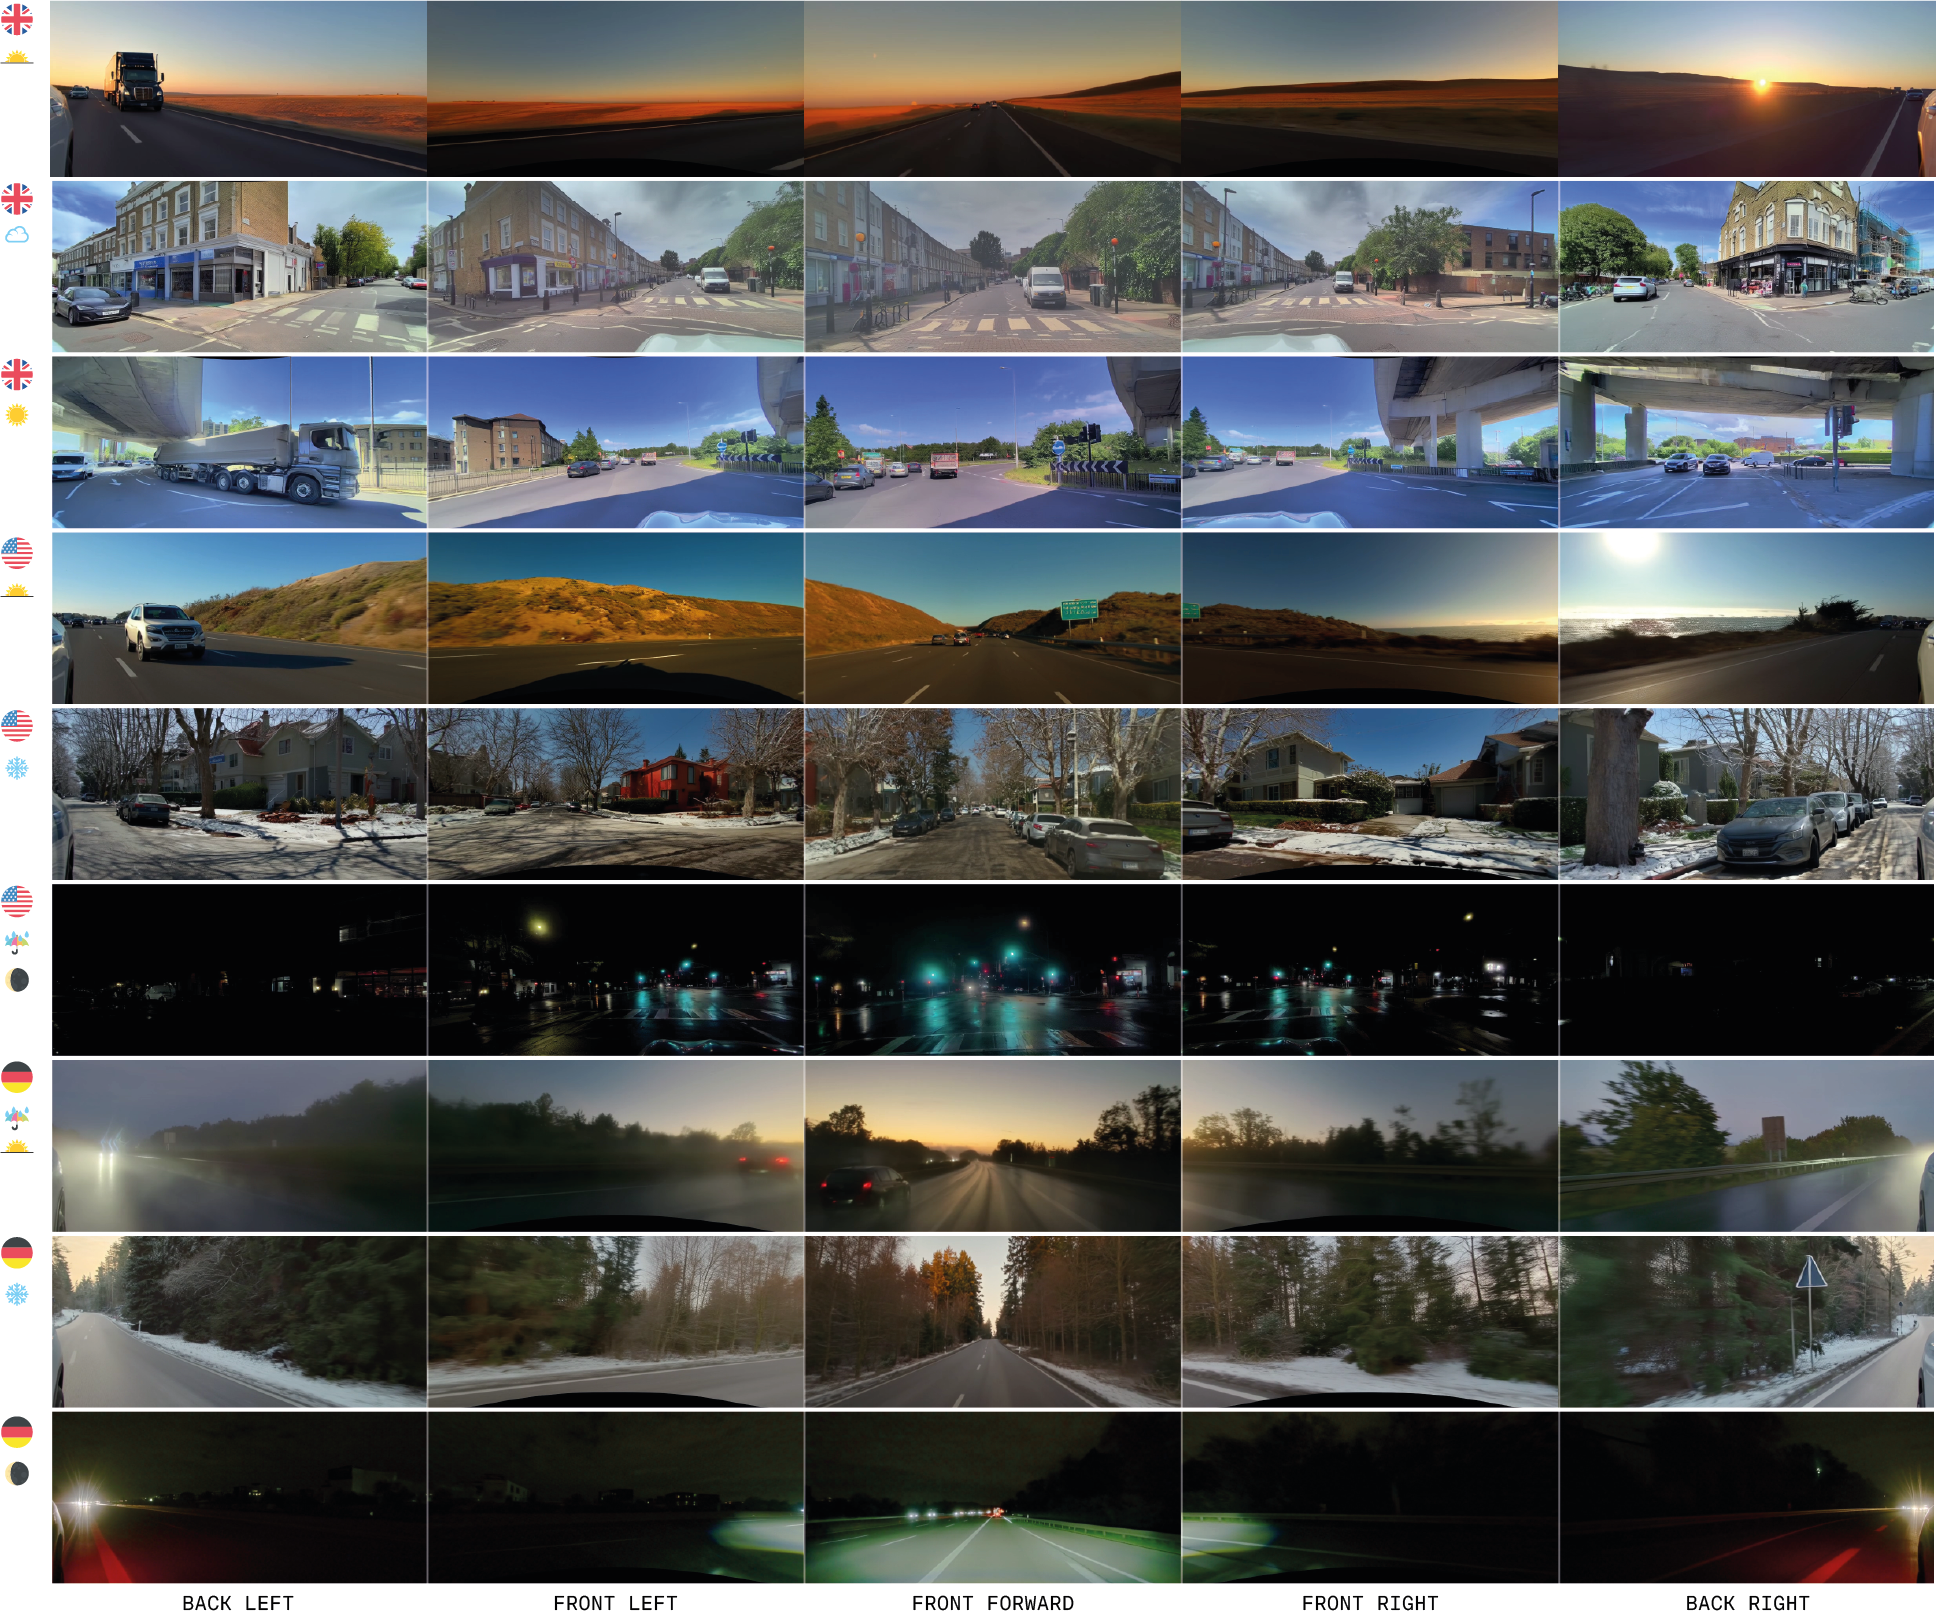
\includegraphics[width=1.0\textwidth]{Figures/diversity_v4_9rows.png}
    \caption{A selection of `\textit{from scratch}' generations demonstrating the diversity of synthetic scenarios possible with GAIA-2.}
    \label{fig:diversity}
    \vspace{-10pt}
\end{figure}

GAIA-2 supports conditioning on a wide range of scene attributes, including ego-vehicle kinematics (e.g., speed, curvature), geographic regions (UK, US, Germany), time of day, weather, and a rich taxonomy of road layout features—such as number and type of lanes (e.g., drivable, bus, cycle), presence of pedestrian crossings, traffic lights, and intersection topology (e.g., one-way roads, roundabouts). It also allows direct control over the locations, orientations, and dimensions of dynamic agents within the scene. This extensive set of conditioning parameters allows for precise control over the generated scenarios, enabling simulation of both typical driving conditions and edge cases critical for robust system evaluation.

To ensure flexibility and interoperability, GAIA-2 enables conditioning on external latent spaces, including CLIP embeddings and a proprietary model trained to produce driving-specific latent representations. This capability allows semantic control over scene content and facilitates integration with downstream planning or perception modules. GAIA-2 further supports multiple video generation modes, including generation from scratch, prediction from past context, and selective content editing through inpainting.

By integrating these capabilities into a single framework, GAIA-2 sets a new benchmark in video-generative world models for autonomous driving. It enables detailed, controllable, and realistic simulation across diverse conditions, providing a powerful tool for scalable training and robust evaluation of autonomous driving systems.